\lab{Python}{Intro to pandas}{Intro to pandas}

In volumes 1 and 2, we solved data problems primarily using NumPy and SciPy.
We now turn our attention to a Python library that is more specifically built for data analysis. Welcome to \emph{pandas}.

\section*{Data Structures in pandas}
Just as NumPy is built on the ndarray data structure suited for efficient scientific and numerical computation, pandas is centered around a handful of core data structures custom built for data analysis. These data structures include the Series, DataFrame, and Panel, which correspond roughly to one-,two-, and three-dimensional arrays. We explore each in turn.

\subsection*{Series}
The Series is a one-dimensional array whose entries are labeled. The values of the array may be
any data type, including integers, strings, or general Python objects. Further, the array
need not be homogeneous. That is, it can hold values of different data types. Together, the array values are referred to as the data of the Series.

The labels must consist of hashable types. They are commonly integers or strings.
Together, the labels are referred to as the index of the Series.

Thus, a Series consists of data and an index. The most basic way to initialize such an object
is as follows:
\begin{lstlisting}
>>> import pandas as pd
>>> s = pd.Series(data, index=index)
\end{lstlisting}
We needn't explicitly define the index. The default index is simply \li{np.arange(len(data))}.

For example, we can create a Series containing the integers from 9 down to 0:
\begin{lstlisting}
>>> s1 = pd.Series(range(9, -1, -1))
>>> s1.values    #the data
array([9, 8, 7, 6, 5, 4, 3, 2, 1, 0], dtype=int64)
>>> s1.index     #the labels
Int64Index([0, 1, 2, 3, 4, 5, 6, 7, 8, 9], dtype='int64')
>>> s1           #left column is index, right column is data
0    9
1    8
2    7
3    6
4    5
5    4
6    3
7    2
8    1
9    0
dtype: int64
\end{lstlisting}

Here is an example where we create customized labels:
\begin{lstlisting}
>>> data = np.random.randn(3)
>>> index = ['first', 'second', 'third']
>>> s2 = pd.Series(data, index=index)
>>> s2
first     1.661255
second   -0.033570
third    -2.185991
dtype: float64
\end{lstlisting}

We can create a Series having constant values in the following manner:
\begin{lstlisting}
>>> val = 4     #desired constant value of Series
>>> n = 6       #desired length of Series
>>> s3 = pd.Series(val, index=range(n))
>>> s3
0    4
1    4
2    4
3    4
4    4
5    4
dtype: int64
\end{lstlisting}

It is also possible to use a Python dict when creating a Series:
\begin{lstlisting}
>>> d = {'e1':93, 'e2':95, 'e3':87, 'e4':82, 'e5':94}
>>> s4 = pd.Series(d)
>>> s4
e1    93
e2    95
e3    87
e4    82
e5    94
dtype: int64
\end{lstlisting}
Note that we didn't need to specify the index: the keys of the dict are used as the index for the Series.

\begin{problem}
Create the following pandas Series.

\begin{itemize}
\item Constant array with value -3, length 5. Labels should be the first five positive even integers.

\item Data is given by the dict \{`Bill':31, `Sarah':28, `Jane':34, `Joe':26\}.
\end{itemize}
\end{problem}

As with the ndarray, we can slice a Series using the usual syntax:
\begin{lstlisting}
>>> s4[:3]
e1    93
e2    95
e3    87
dtype: int64
\end{lstlisting}
Notice that both the data and the index are sliced in this manner.
We can also input Series with numerical data into many NumPy functions.
\begin{lstlisting}
>>> np.log(s4)
e1    4.532599
e2    4.553877
e3    4.465908
e4    4.406719
e5    4.543295
dtype: float64
\end{lstlisting}

A Series also has similarities with the Python dict.
We can access and alter the data using the index.
\begin{lstlisting}
>>> s4['e3']
87
>>> s4['e3'] = 99
>>> s4['e3']
99
\end{lstlisting}

We finish off this section by considering elementary vectorized operations with Series.
\begin{lstlisting}
>>> x = pd.Series(np.random.randn(4), index=['a', 'b', 'c', 'd'])
>>> x
a   -0.924259
b    0.767422
c    0.399212
d    0.130365
dtype: float64
>>> y = pd.Series(np.random.randn(5), index=['a', 'b', 'd', 'e', 'f'])
>>> y
a   -0.708301
b   -2.214516
d   -2.352364
e    0.789419
f   -0.859482
dtype: float64
\end{lstlisting}
Much as with the NumPy array, we can perform basic arithmetic operations on the entries of
a Series without the use of a for-loop. For example, we square the elements of \li{x} as
follows:
\begin{lstlisting}
>>> x**2
a    0.854254
b    0.588937
c    0.159370
d    0.016995
dtype: float64
\end{lstlisting}
In some cases, the Series allows for even greater flexibility than the NumPy array. For example,
we are able to add Series \li{x} and \li{y}, even though they have different lengths and labels:
\begin{lstlisting}
>>> z = x+y
>>> z
a   -1.632559
b   -1.447093
c         NaN
d   -2.221999
e         NaN
f         NaN
dtype: float64
\end{lstlisting}
Notice that the index of \li{z} is the \emph{union} of the index of \li{x} and the index of \li{y}.
For the labels shared by both \li{x} and \li{y} (namely \li{a}, \li{b}, and \li{d}), the corresponding
value of \li{z} is just the sum of the entries of \li{x} and \li{y}. In all other cases, the value of
\li{z} is \li{NaN}, which is the pandas type indicating a missing value. It is simple to omit missing
values from a series:
\begin{lstlisting}
>>> z.dropna()
a   -1.632559
b   -1.447093
d   -2.221999
dtype: float64
\end{lstlisting}




\subsection*{DataFrame}
The DataFrame data structure is a two-dimensional generalization of the Series. It can be viewed
as a tabular structure with labeled rows and columns. The row labels are collectively called the
index, and the column labels are collectively called the columns. An individual column in a
DataFrame object is a Series.

There are many ways to initialize a DataFrame. In the following, we build a DataFrame out of a
dict of Series.
\begin{lstlisting}
>>> d = {1:x, 2:y}
>>> df1 = pd.DataFrame(d)
>>> df1
	        1	        2
a	-0.924259	-0.708301
b	 0.767422	-2.214516
c	 0.399212	      NaN
d	 0.130365	-2.352364
e	      NaN	 0.789419
f	      NaN	-0.859482
\end{lstlisting}
Note that the index of this DataFrame is the union of the index of Series \li{x} and that of Series \li{y}.
The columns are given by the keys of the dict \li{d}. Since \li{x} doesn't have a label \li{e}, the
value in row \li{e}, column \li{1} is \li{NaN}. This same reasoning explains the other missing values as well.
Note that if we take the first column of the DataFrame and drop the missing values, we recover the Series \li{x}:
\begin{lstlisting}
>>> x == df1[1].dropna()
a    True
b    True
c    True
d    True
dtype: bool
\end{lstlisting}

We can also initialize a DataFrame using a NumPy array, creating custom row and column labels:
\begin{lstlisting}
>>> data = np.random.random((3,4))
>>> pd.DataFrame(data, index=['A','B','C'], columns=range(1,5))

            1	        2	        3	        4
A	 0.065646	 0.968593	 0.593394	 0.750110
B	 0.803829	 0.662237	 0.200592	 0.137713
C	 0.288801	 0.956662	 0.817915	 0.951016
3 rows � 4 columns
\end{lstlisting}
As with Series, if we don't specify the index or columns, the default is \li{range(n)}, where \li{n} is either the number of
rows or columns.

It is also possible to create multi-indexed arrays, for example
\begin{lstlisting}
>>> grade=['eighth','ninth','tenth']
>>> subject=['math','science','english']
>>> myindex = pd.MultiIndex.from_product([grade,subject], names=['grade','subje
t'])
>>> myseries = pd.Series(np.random.randn(9),index=myindex)
>>> myseries
grade   subject
eighth  math       1.706644
        science   -0.899587
        english   -1.009832
ninth   math       2.096838
        science    1.884932
        english    0.413266
tenth   math      -0.924962
        science   -0.851689
        english    1.053329
dtype: float64
\end{lstlisting}

Multi-indexing is visually convenient, but not strictly necessary for most applications. The interested reader is invited to explore the documentation to learn more.

A DataFrame behaves in certain respects like a dict of Series, where each column label and the corresponding column form the key-value pairs.
We can access a desired column via its column label:
\begin{lstlisting}
>>> df1[2]
a   -0.708301
b   -2.214516
c         NaN
d   -2.352364
e    0.789419
f   -0.859482
Name: 2, dtype: float64
\end{lstlisting}
We can insert a new column or delete a column much as we would with a dict:
\begin{lstlisting}
>>> df1['product'] = df1[1] * df1[2]  #insert column containing the product of columns 1 and 2
>>> df1['constant'] = 'const'         #insert column containing constant data
>>> df1
            1	        2	  product	 constant
a	-0.924259	-0.708301	 0.654653	    const
b	 0.767422	-2.214516	-1.699469	    const
c	 0.399212	      NaN	      NaN	    const
d	 0.130365	-2.352364	-0.306666	    const
e	      NaN	 0.789419	      NaN	    const
f	      NaN	-0.859482	      NaN	    const
6 rows � 4 columns
>>> del df1['constant']
            1	        2	  product	
a	-0.924259	-0.708301	 0.654653	
b	 0.767422	-2.214516	-1.699469	
c	 0.399212	      NaN	      NaN	
d	 0.130365	-2.352364	-0.306666	
e	      NaN	 0.789419	      NaN	
f	      NaN	-0.859482	      NaN	
6 rows � 4 columns
\end{lstlisting}

We can also select specified rows, either using the row label, or its integer position:
\begin{lstlisting}
>>> df1.loc['b']        #select 2nd row via label
1          0.767422
2         -2.214516
product   -1.699469
Name: b, dtype: float64
>>> df1.iloc[1]         #select 2nd row via integer position
1          0.767422
2         -2.214516
product   -1.699469
Name: b, dtype: float64
\end{lstlisting}
We can slice rows much as we do with NumPy arrays:
\begin{lstlisting}
>>> df1[1:4]
	        1	        2	  product
b	 0.767422	-2.214516	-1.699469
c	 0.399212	      NaN	      NaN
d	 0.130365	-2.352364	-0.306666
3 rows � 3 columns
\end{lstlisting}

A particularly slick way to slice rows is by boolean indexing, in which a criterion for selecting rows is given.

\begin{lstlisting}
>>> df #Here's a data frame
           A         B         C strcol
0   0.628435  1.910799  0.194874   asdf
1   0.785914  0.412298 -1.813564   asdf
2   1.124251  0.929658 -0.580788   asdf
3   0.978128  1.126996 -0.063130   asdf
4   0.529262  1.063394  0.304336   asdf
5  -0.310556 -0.012804 -1.042040   asdf
6  -0.561364  0.382025 -1.103540   asdf
7   1.335368  0.676128  0.101528   asdf
8  -0.315294 -0.273289 -0.009816   asdf
9   0.179279  0.743868  0.294675   asdf
10  0.694140 -0.808863  1.243764   asdf
11 -0.811642  2.499150  2.100622   asdf
12  0.834592 -0.197040 -0.133127   asdf

[212 rows x 4 columns]
>>> df[df['C']>0] #Get all the rows of df for which the element in the C column is positive.
           A         B         C strcol
0   0.628435  1.910799  0.194874   asdf
4   0.529262  1.063394  0.304336   asdf
7   1.335368  0.676128  0.101528   asdf
9   0.179279  0.743868  0.294675   asdf
10  0.694140 -0.808863  1.243764   asdf
11 -0.811642  2.499150  2.100622   asdf
[6 rows x 4 columns]
\end{lstlisting}

Boolean indexing is particularly useful for selecting data that satisfy certain criteria, including when it comes time for data cleaning. One caution: if multiple statements are used to select rows, they must be separated by parenthesis:

\begin{lstlisting}
>>> df[(df['C']>0) & (df['A']> 0.3)] #Note the parenthesis
           A         B         C strcol
0   0.628435  1.910799  0.194874   asdf
4   0.529262  1.063394  0.304336   asdf
7   1.335368  0.676128  0.101528   asdf
10  0.694140 -0.808863  1.243764   asdf
15  0.594757 -0.659265  0.023030   asdf

[5 rows x 4 columns]
>>> df[df['C']>0 & df['A']> 0.3] #Forgot parenthesis. This will cause an error.
\end{lstlisting}

\subsection*{Panel}



The third fundamental object in \li{pandas} is ``Panel.'' It is analogous to a three-dimensional array and was designed for dealing with panel data, which is common in economic research, among other fields. In economics, for instance, one might want to track information for several countries over multiple years. Panel is the least-commonly used of the three fundamental pandas datatypes, but it is worth knowing about.

The three axes of a Panel are \li{items}, \li{major_axis}, and \li{minor_axis}, so a panel can be initialized from a 3-dimensional array as follows:

\begin{lstlisting}
pan = pd.Panel(np.random.randn(3,2,3), items=['1','2','3'],major_axis=['A','B'],minor_axis=['a','b','c'])
\end{lstlisting}

To see what this looks like, use the command \li{to_frame}, which lists out the data as a multi-indexed DataFrame.

\begin{lstlisting}
>>> pan = pd.Panel(np.random.randn(3,2,3), items=['1','2','3'],major_axis=['A',
B'],minor_axis=['a','b','c'])
>>> pan
<class 'pandas.core.panel.Panel'>
Dimensions: 3 (items) x 2 (major_axis) x 3 (minor_axis)
Items axis: 1 to 3
Major_axis axis: A to B
Minor_axis axis: a to c
>>> pan.to_frame()
                    1         2         3
major minor
A     a     -0.252654 -0.913452 -0.901322
      b      1.933009 -0.262968 -0.467978
      c      0.484946 -0.214478 -0.061904
B     a     -0.959360  2.475628  0.900854
      b      0.257859 -0.879048 -1.243879
      c     -0.103787 -1.141230  0.222686

[6 rows x 3 columns]
\end{lstlisting}

Alternatively, a panel can be constructed from a dict of DataFrames, as follows:

\begin{lstlisting}
paneldata = {'2001' : pd.DataFrame(np.random.randn(2, 3)),
'2011' : pd.DataFrame(np.random.randn(3, 2))}
paneldata=pd.Panel(paneldata)
\end{lstlisting}

The operation above deals nicely with the asymmetric data, inserting \li{NaN}, where needed. If you want to view the panel using \li{to_frame}, however, the default is to drop the asymmetric parts and reduce to a $2\times 2\times 2$ structure. Another way to access the data in a particular item is simply to use \li{paneldata['2011']}.

Many of the functions of the DataFrame type perform similarly on the Panel type. These include transposition, adding/deleting items, and accessing data. Another way to use panel is to use \li{squeeze} to

\section*{Viewing Data}

\subsection*{Plotting}

Another way of viewing your data is through the plotting functionalities. Fortunately, this is just done through \li{matplotlib}, without much modification. Here are some examples, the first two of which are from the pandas documentation

\begin{lstlisting}
>>> import matplotlib.pyplot as plt
>>> s=pd.Series(np.random.randn(1000))
>>> s=s.cumsum()
>>> plt.plot(s)
[<matplotlib.lines.Line2D object at 0x000000000A185208>]
>>> plt.show()
\end{lstlisting}

Here's the output:

\begin{figure}
\centering
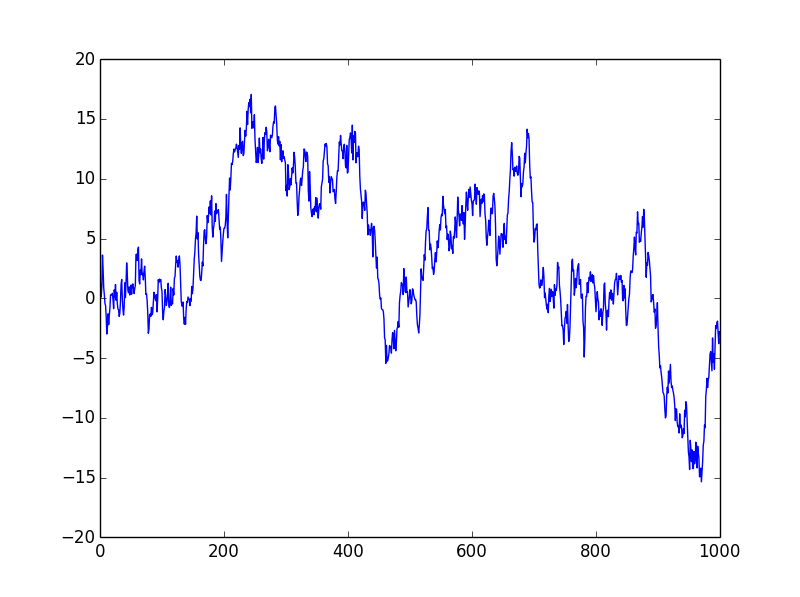
\includegraphics[width=.5 \textwidth]{cumsumplot.png}
\caption{ Graph of s.
}
\label{pandas:cumsumplot}
\end{figure}

\begin{problem}
Run the above code 5 times to get 5 images. Then change the number of steps to 100 and to 10,000. What happens to the max/min and number of ``big'' peaks and troughs when the scale changes? (If you're really clever, you can guess how this would generalize to arbitrarily long series.)
\end{problem}

Using DataFrames, one can also plot one column against another.

\begin{lstlisting}
>>> import matplotlib.pyplot as plt #Need this to plot
>>> xvals=pd.Series(range(1000))
>>> xvals=np.sqrt(xvals) #Make some interesting x-values
>>> yvals=pd.Series(np.random.randn(1000).cumsum()) #And interesting y-values
>>> df=pd.DataFrame({'xvals':xvals,'yvals':yvals}) #Put in in a dataframe
>>> df.plot(x='xvals',y='yvals') #Plot, specifying which column is to be used to x and y values. A reference is returned.
<matplotlib.axes.AxesSubplot object at 0x000000000B459320>
>>> plt.show() #Look at it!
\end{lstlisting}

Here's the output:

\begin{figure}
\centering
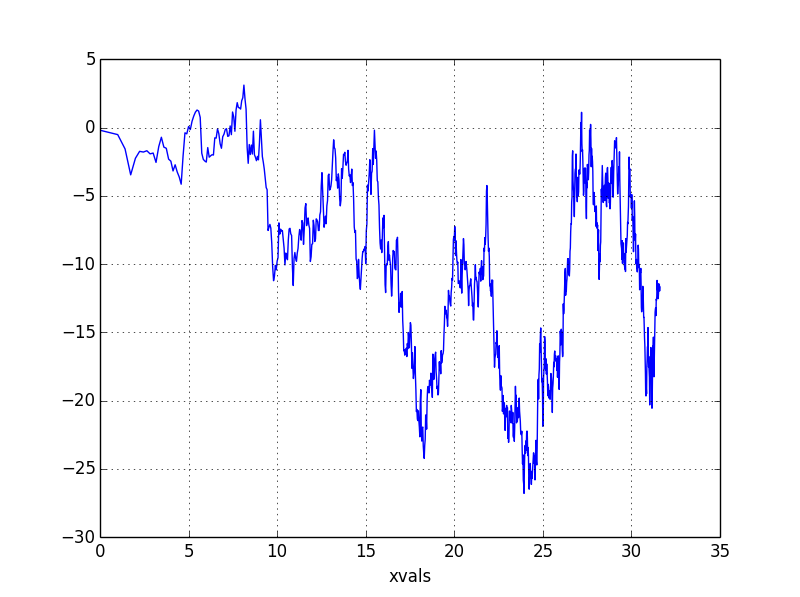
\includegraphics[width=.5 \textwidth]{cumsumplot1.png}
\caption{ Graph generated when one coordinate is taken from the xvals column and the other from the yvals column.
}
\label{pandas:cumsumplot1}
\end{figure}

A variety of other types of plots are possible. Here's a histogram:

\begin{lstlisting}
>>> df['yvals'].diff().hist() #Using the same df as in the previous example, takes the yvals column and makes a histogram.
<matplotlib.axes.AxesSubplot object at 0x000000000B4696D8>
>>> plt.show()
\end{lstlisting}

Here's the output:

\begin{figure}
\centering
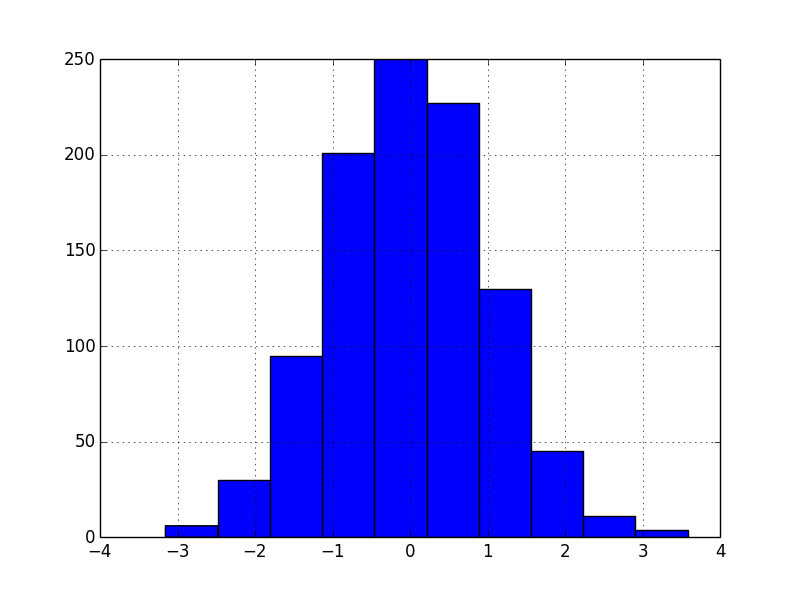
\includegraphics[width=.5 \textwidth]{cumsumplot2.png}
\caption{ Histogram of the y-values of df.
}
\label{pandas:cumsumplot2}
\end{figure}




\subsection*{SQL Joins and Selects}

One of the advantages of pandas is that it has high-powered implementations of some central SQL operations, thus reducing the temptation to switch between programming languages for different tasks. For instance, all major types of joins are supported. Here are some examples:

\begin{lstlisting}
>>> df1 #First data frame
      DATA1     DATA2  EMPLOYEEID
0  0.763628  0.671691           1
1  0.635869  1.486546           2
2  1.917649 -0.432400           3
3 -0.679496  0.794938           4
4 -0.201446  1.936673           5

[5 rows x 3 columns]
>>> df2 #Second data frame
      DATA3     DATA4  EMPLOYEEID
0 -1.194058  0.814376           2
1  1.068904 -0.289241           3
2  0.099272  0.595524           4
3  0.688357 -0.207746           5
4  0.292399  0.504268           6
5 -0.259372  1.159809           7

[6 rows x 3 columns]
>>> pd.merge(df1,df2,on='EMPLOYEEID') #Use the merge function to do SQL joins. The default is inner join.
      DATA1     DATA2  EMPLOYEEID     DATA3     DATA4
0  0.635869  1.486546           2 -1.194058  0.814376
1  1.917649 -0.432400           3  1.068904 -0.289241
2 -0.679496  0.794938           4  0.099272  0.595524
3 -0.201446  1.936673           5  0.688357 -0.207746

[4 rows x 5 columns]
>>> pd.merge(df1,df2,on='EMPLOYEEID',how='outer') #The how keyword allows for the other major join types. Notice how NaN is used to fill missing spots.
      DATA1     DATA2  EMPLOYEEID     DATA3     DATA4
0  0.763628  0.671691           1       NaN       NaN
1  0.635869  1.486546           2 -1.194058  0.814376
2  1.917649 -0.432400           3  1.068904 -0.289241
3 -0.679496  0.794938           4  0.099272  0.595524
4 -0.201446  1.936673           5  0.688357 -0.207746
5       NaN       NaN           6  0.292399  0.504268
6       NaN       NaN           7 -0.259372  1.159809

[7 rows x 5 columns]
>>> pd.merge(df1,df2,on='EMPLOYEEID',how='left') #Left outer join
      DATA1     DATA2  EMPLOYEEID     DATA3     DATA4
0  0.763628  0.671691           1       NaN       NaN
1  0.635869  1.486546           2 -1.194058  0.814376
2  1.917649 -0.432400           3  1.068904 -0.289241
3 -0.679496  0.794938           4  0.099272  0.595524
4 -0.201446  1.936673           5  0.688357 -0.207746

[5 rows x 5 columns]
>>> pd.merge(df1,df2,on='EMPLOYEEID',how='right') #Right outer join
      DATA1     DATA2  EMPLOYEEID     DATA3     DATA4
0  0.635869  1.486546           2 -1.194058  0.814376
1  1.917649 -0.432400           3  1.068904 -0.289241
2 -0.679496  0.794938           4  0.099272  0.595524
3 -0.201446  1.936673           5  0.688357 -0.207746
4       NaN       NaN           6  0.292399  0.504268
5       NaN       NaN           7 -0.259372  1.159809

[6 rows x 5 columns]
\end{lstlisting}

The SQL command \li{select} also has an easy substitute.

\begin{lstlisting}
>>> df1[['EMPLOYEEID','DATA1']] #Select only two of the columns
   EMPLOYEEID     DATA1
0           1  0.763628
1           2  0.635869
2           3  1.917649
3           4 -0.679496
4           5 -0.201446

[5 rows x 2 columns]
>>> df1[['EMPLOYEEID','DATA1']].head(2) #Take only the first two rows
   EMPLOYEEID     DATA1
0           1  0.763628
1           2  0.635869

[2 rows x 2 columns]
>>> df1[['EMPLOYEEID','DATA1']].tail(3) #Take only the last three rows
   EMPLOYEEID     DATA1
2           3  1.917649
3           4 -0.679496
4           5 -0.201446

[3 rows x 2 columns]
\end{lstlisting}

\section*{Manipulating Data}

Pandas is particularly well-suited to handling missing and anomalous data. The pandas default for a missing value is \li{NaN}. In basic arithmetic operations, missing values are dealt with in a conservative manner:

\begin{lstlisting}
>>> myseries2 = pd.Series(np.random.randn(9),index=myindex)
>>> myseries2['eighth','english']='NaN'
>>> myseries2
grade   subject
eighth  math       0.191243
        science    0.554761
        english         NaN
ninth   math      -0.526643
        science    2.398025
        english    1.082043
tenth   math       1.396143
        science   -0.850942
        english   -1.378125
dtype: float64
>>> myseries
grade   subject
eighth  math       1.706644
        science   -0.899587
        english   -1.009832
ninth   math       2.096838
        science    1.884932
        english    0.413266
tenth   math      -0.924962
        science   -0.851689
        english    1.053329
dtype: float64
>>> myseries+myseries2
grade   subject
eighth  math       1.897887
        science   -0.344826
        english         NaN
ninth   math       1.570195
        science    4.282957
        english    1.495309
tenth   math       0.471181
        science   -1.702631
        english   -0.324795
dtype: float64
\end{lstlisting}

Other functions, such as $.sum()$ and $.mean()$ treat NaN as zero.

\begin{lstlisting}
>>> myseries2.mean()
0.35831305133218083
\end{lstlisting}

There are several ways to deal with NaN entries. One is to simply drop them.

\begin{lstlisting}
>>> myseries2.dropna()
grade   subject
eighth  math       0.191243
        science    0.554761
ninth   math      -0.526643
        science    2.398025
        english    1.082043
tenth   math       1.396143
        science   -0.850942
        english   -1.378125
dtype: float64
\end{lstlisting}

Notice that the above operation did not chance myseries2, but rather created a new series without the NaN entries. To change myseries2 directly, use the inplace option

\begin{lstlisting}
>>> myseries3.dropna(inplace=True)
\end{lstlisting}

Alternately, rather than dropping NaN entries, it might be suitable to replace them with the mean or some other value.

\begin{lstlisting}
>>> myseries2.fillna(myseries2.mean())
grade   subject
eighth  math       0.191243
        science    0.554761
        english    0.358313
ninth   math      -0.526643
        science    2.398025
        english    1.082043
tenth   math       1.396143
        science   -0.850942
        english   -1.378125
dtype: float64
>>> myseries2.mean()
0.35831305133218083
\end{lstlisting}

Other ``cleaning'' operations include transposing and sorting. ``Transposing'' means flipping the rows and columns (see example below), and sorting is simply ordering the data in some meaningful way.

\begin{lstlisting}
>>> df #Original dataframe
            0         1         2         3         4
a 0 -1.749534  0.763194  1.039742 -1.179616  2.128509
b 1 -0.956593 -0.032001  1.249905  0.418494 -0.029238
c 2  0.485885 -1.539459 -0.602270  1.939523  0.291494
d 3 -1.328571       NaN  0.481167  1.623820  0.228658
e 4  1.731380  1.395385 -0.207489  0.253467  0.348348

[5 rows x 5 columns]
>>> df.transpose() #Transposed dataframe. See how the rows and columns are switched?
          a         b         c         d         e
          0         1         2         3         4
0 -1.749534 -0.956593  0.485885 -1.328571  1.731380
1  0.763194 -0.032001 -1.539459       NaN  1.395385
2  1.039742  1.249905 -0.602270  0.481167 -0.207489
3 -1.179616  0.418494  1.939523  1.623820  0.253467
4  2.128509 -0.029238  0.291494  0.228658  0.348348

[5 rows x 5 columns]

#Now let's sort the data
>>> mydata #Original DataFrame
          0         1         2         3
a -1.150876  0.201994 -0.447484 -0.204217
b -0.171968 -0.303143 -0.605779  0.499296
c -0.647877 -0.010989  0.881816 -0.783891
d  1.500841  0.698213  0.963573  0.964841
e -0.274085 -0.124850  0.947559  0.697708

[5 rows x 4 columns]
>>> mydata.sort([1]) #Sorted by the entries of column 1
          0         1         2         3
b -0.171968 -0.303143 -0.605779  0.499296
e -0.274085 -0.124850  0.947559  0.697708
c -0.647877 -0.010989  0.881816 -0.783891
a -1.150876  0.201994 -0.447484 -0.204217
d  1.500841  0.698213  0.963573  0.964841

[5 rows x 4 columns]
\end{lstlisting}

With these basic ideas and operations in hand, you'll be prepared to deal with the missing values and formatting indiscrepancies that occur in most real-life data sets.

\section*{Analyzing Data}

Of course, the whole point of \li{pandas} is to help you \emph{analyze} the data once it's inputted. Several upcoming labs will involve practicing different ways of using pandas for data analysis. We'll just cover the very basics right now.

A good first step is just to determine the datatypes of each column in a data frame:

\begin{lstlisting}
>>> df['a'][0]='this' #Changing this entry to make the DataFrame more interesting.
>>> df
           a         b         c         d         e
0       this -0.171968 -0.647877  1.500841 -0.274085
1  0.2019935 -0.303143 -0.010989  0.698213 -0.124850
2 -0.4474842 -0.605779  0.881816  0.963573  0.947559
3 -0.2042165  0.499296 -0.783891  0.964841  0.697708

[4 rows x 5 columns]
>>> df.info() #Asking for the contents of each column.
<class 'pandas.core.frame.DataFrame'>
Int64Index: 4 entries, 0 to 3
Data columns (total 5 columns):
a    4 non-null object #Notice this one.
b    4 non-null float64
c    4 non-null float64
d    4 non-null float64
e    4 non-null float64
dtypes: float64(4), object(1)
\end{lstlisting}

It is worth noting that the datatypes in each column need not be homogenous, in which case, the classification is given simply as ``object.''

Another quick, easy analysis is given by the \li{describe} method.

\begin{lstlisting}
>>> df.describe()
              b         c         d         e
count  4.000000  4.000000  4.000000  4.000000 #Number of entries per column
mean  -0.145398 -0.140235  1.031867  0.311583 #Mean
std    0.466608  0.760107  0.336857  0.601952 #Standard deviation
min   -0.605779 -0.783891  0.698213 -0.274085 #The five number summary
25%   -0.378802 -0.681881  0.897233 -0.162158
50%   -0.237555 -0.329433  0.964207  0.286429
75%   -0.004152  0.212212  1.098841  0.760171
max    0.499296  0.881816  1.500841  0.947559
\end{lstlisting}

There are also easy commands to get covariance matrices (.cov()), correlation matices (.corr()), and almost any other basic statistical info.



\section*{Data I/O}

Before we can use \li{pandas} for anything, we need to have some data, and when we're done using the data, we need to store it in a convenient place and format. In other words, we need to do data input/output, or I/O. The process of input is called \textit{reading}, and the process of output is called \textit{writing}. Reading usually takes data from another file, such as a CSV file, and turns it into a \li{python} data type. Writing then creates or updates another file with the most recent configuration of the data.\\
\indent The \li{pandas} package supports reading many different file types, using functions such as \li{pd.read_csv(),pd.read_stata(), pd.read_excel()}, etc. The output is a DataFrame object, although there is an option, \li{squeeze}, to make the output a Series object. For instance, to read a \li{.csv} file, one could use the following code:
\begin{lstlisting}
pd.read_csv('FakeData.csv', index_col=0)
\end{lstlisting}
Here, the first argument gives the file name, and the second specifies that the first column be used to index the table. If the second argument is left off, python will generate its own index column. Here's the output:

\begin{lstlisting}
           date  time  room instructor
Psych  20120101  1200    12    Carlson
Math   20120102   100    14      Smith
Bio    20120378   400    17   Hamilton

[3 rows x 4 columns]
\end{lstlisting}

Compare this with the output we get without \li{pandas}
\begin{lstlisting}
>>> print(open('C:\...\FakeData.csv').read())
,date,time,room,instructor
Psych,20120101,1200,12,Carlson
Math,20120102,100,14,Smith
Bio,20120378,400,17,Hamilton
\end{lstlisting}

Not nearly as structured or easy to interpret!

Many real-world data sets contain imperfections that you will need to ``clean,'' and some of these issues will need to be cleared up at the time that the data is read in. For instance, while \li{pandas} has some ability to read in data sets with missing values, it will generally need your help (possibly in the form of the \li{error_bad_lines} option) to handle a line of data with extra values. Because there are so many possible problems with reading in real data, the reader is encouraged to look through the documentation when specific issues arise.\\
\indent Writing tends to be much less messy since the data is already going to be in a format suitable for computations. The only details that typically come up are in specifying what formatting should be put on the output file. There are many options attached to the write commands, such as whether to include headers, and which options are specified depends on the future use that the data will have. Most of the time, a write command will just look like this:
\begin{lstlisting}
mydatatable.to_csv('FakeData1.csv')
\end{lstlisting}

\begin{problem}
Download the dataset at \url{http://research.stlouisfed.org/fred2/series/ACILACB#}, which is some loan data put together by the St. Louis Fed. It will be an Excel file. Use the command \li{pd.read_excel} to read in the file. Notice that this command takes two arguments, the path to the file and the name of the sheet to be read. Look at the resulting DataFrame. It probably won't look very good due to the presence of extra information in the file. One easy way to fix this is just to open the Excel file, manually remove the extra material, and read the file again. Do this, and look at the results. The DataFrame should look much neater now. Use the \li{describe} command to get the mean of the data.\\

Now, the data presented here is quarterly. Reduce the data by removing all except for the January data. Write this to a file, ``fradgraph2.xls,'' and turn the file in, along with the mean calculated, as above.
\end{problem}













































